\svnInfo $Id$
\chapter{Analysis fields}\label{sec_analysis}

The 3-hourly first guess output of ICON contains the following fields:

\begin{longtable}{p{4.0cm}P{7.0cm}}
\caption[]{Available 3h first guess output fields}\\
  \toprule
\multicolumn{1}{c}{\textbf{Type}}  &  \multicolumn{1}{c}{\textbf{GRIB shortName}}\\
\midrule
\endfirsthead
\caption[]{\emph{continued}}\\
\midrule
\endhead
\hline \multicolumn{2}{r}{\textit{Continued on next page}} \\
\endfoot
\endlastfoot
Atmosphere                             &  VN, U, V, W, DEN, THETA\_V, T, QV, QC, QI, QR, QS, TKE, P                     \\
Surface (general)                      &  T\_G, T\_SO(0), QV\_S, T\_2M, TD\_2M, U\_10M, V\_10M, PS, Z0                       \\
Land specific                          &  W\_SNOW, T\_SNOW, RHO\_SNOW, H\_SNOW, FRESHSNW, W\_I, T\_SO(1:nlev\_soil), W\_SO, W\_SO\_ICE \\
Lake/sea ice specific                  &  T\_MNW\_LK, T\_WML\_LK, H\_ML\_LK, T\_BOT\_LK, C\_T\_LK, T\_B1\_LK, H\_B1\_LK, T\_ICE, H\_ICE, FR\_ICE\\
Time invariant                         &  FR\_LAND, HHL, CLON, CLAT, ELON, ELAT, VLON, VLAT \\
  \bottomrule
\end{longtable}

Atmospheric analysis fields are computed every 3 hours ($00$, $03$, $06$,$\dots$ $21$ UTC) by the 3DVar data assimilation system. Sea surface 
temperature \texttt{T\_SO(0)} and sea ice cover \texttt{FR\_ICE} are provided once per day (00 UTC) by the SST-Analysis. A snow analysis is 
conducted every 3 hours, providing updated information on the snow height \texttt{H\_SNOW} and snow age \texttt{FRESHSNW}. In addition a soil 
moisture analysis (SMA) is conducted once per day (00 UTC). It basically modifies the soil moisture content \texttt{W\_SO}, in order to improve 
the $2\,\mathrm{m}$ temperature forecast. 

 
For the 3-hourly assimilation cycle and forecast runs, ICON must be provided with $2$ input files: One containing the First Guess~(FG) and the other 
containing analysis~(AN) fields, only. Variables for which no analysis is available are always read from the first guess file (e.g.\ TKE). 
Other variables may be read either from the first guess or the analysis file, depending on the starting time. E.g.\ for T\_SO(0) the first 
guess is read at 03, 06, 09, 12, 15, 18, 21 UTC, however, the analyis is read at 00 UTC when a new SST analysis is available. 
In Table~\ref{tbl_analysis} the available and employed first guess and analysis fields are listed as a function of starting time.

\begin{longtable}{p{3.3cm}>{\centering\arraybackslash}p{2.5cm}p{0.7cm}p{0.7cm}p{0.7cm}p{0.7cm}p{0.7cm}p{0.7cm}p{0.7cm}p{0.7cm}}
\caption[]{The leftmost column shows variables that are mandatory for the assimilation cycle and forecast runs.  Column 2 indicates, whether or not an analysis is performed 
for these variables. Columns 3 to 10 show the origin of these variables (analysis or first guess), depending on the starting time.}\label{tbl_analysis}\\
  \toprule
\textbf{ShortName}  &  \textbf{Analysis}  & \textbf{00} & \textbf{03} & \textbf{06} & \textbf{09} & \textbf{12} & \textbf{15} & \textbf{18} &  \textbf{21} \\
\midrule
\endhead
\hline \multicolumn{10}{r}{\textit{Continued on next page}} \\
\endfoot
\endlastfoot
\hline \multicolumn{10}{l}{\textbf{Atmosphere}} \\
VN                  &     --              &   FG         &     FG      &     FG      &     FG      &     FG      &     FG      &     FG      &    FG         \\
THETA\_V            &     --              &   FG         &     FG      &     FG      &     FG      &     FG      &     FG      &     FG      &    FG         \\
DEN                 &     --              &   FG         &     FG      &     FG      &     FG      &     FG      &     FG      &     FG      &    FG         \\
W                   &     --              &   FG         &     FG      &     FG      &     FG      &     FG      &     FG      &     FG      &    FG         \\
TKE                 &     --              &   FG         &     FG      &     FG      &     FG      &     FG      &     FG      &     FG      &    FG         \\
QC, QI, QR, QS      &     --              &   FG         &     FG      &     FG      &     FG      &     FG      &     FG      &     FG      &    FG         \\
QV                  &     3DVar           &   \tred{AN}  &  \tred{AN}  &  \tred{AN}  &   \tred{AN} &   \tred{AN} &  \tred{AN}  &  \tred{AN}  &  \tred{AN}    \\
T                   &     3DVar           &   \tred{AN}  &  \tred{AN}  &  \tred{AN}  &   \tred{AN} &   \tred{AN} &  \tred{AN}  &  \tred{AN}  &  \tred{AN}    \\
P                   &     3DVar           &   \tred{AN}  &  \tred{AN}  &  \tred{AN}  &   \tred{AN} &   \tred{AN} &  \tred{AN}  &  \tred{AN}  &  \tred{AN}    \\
U, V                &     3DVar           &   \tred{AN}  &  \tred{AN}  &  \tred{AN}  &   \tred{AN} &   \tred{AN} &  \tred{AN}  &  \tred{AN}  &  \tred{AN}    \\
\hline \multicolumn{10}{l}{\textbf{Surface}} \\
Z0                  &     --              &   FG         &     FG      &     FG      &     FG      &     FG      &     FG      &     FG      &    FG         \\
T\_G                &     --              &   FG         &     FG      &     FG      &     FG      &     FG      &     FG      &     FG      &    FG         \\
QV\_S               &     --              &   FG         &     FG      &     FG      &     FG      &     FG      &     FG      &     FG      &    FG         \\
T\_SO(0) (SST only) &    Ana\_SST         &   \tred{AN}  &     FG      &     FG      &     FG      &     FG      &     FG      &     FG      &    FG         \\
T\_SO(0:nlevsoil)   &     --              &   FG         &     FG      &     FG      &     FG      &     FG      &     FG      &     FG      &    FG         \\
W\_SO\_ICE          &     --              &   FG         &     FG      &     FG      &     FG      &     FG      &     FG      &     FG      &    FG         \\
W\_SO               &      SMA            &   \tred{AN}  &     FG      &     FG      &     FG      &     FG      &     FG      &     FG      &    FG         \\
W\_I                &      --             &   FG         &     FG      &     FG      &     FG      &     FG      &     FG      &     FG      &    FG         \\
W\_SNOW\footnotemark[1] &    Ana\_SNOW    &   \tred{AN}  &  \tred{AN}  &  \tred{AN}  &   \tred{AN} &   \tred{AN} &  \tred{AN}  &  \tred{AN}  &  \tred{AN}    \\
T\_SNOW             &      --             &   FG         &     FG      &     FG      &     FG      &     FG      &     FG      &     FG      &    FG         \\
RHO\_SNOW\footnotemark[1] &    Ana\_SNOW  &   \tred{AN}  &  \tred{AN}  &  \tred{AN}  &   \tred{AN} &   \tred{AN} &  \tred{AN}  &  \tred{AN}  &  \tred{AN}    \\
H\_SNOW             &    Ana\_SNOW        &   \tred{AN}  &  \tred{AN}  &  \tred{AN}  &   \tred{AN} &   \tred{AN} &  \tred{AN}  &  \tred{AN}  &  \tred{AN}    \\
FRESHSNW            &    Ana\_SNOW        &   \tred{AN}  &  \tred{AN}  &  \tred{AN}  &   \tred{AN} &   \tred{AN} &  \tred{AN}  &  \tred{AN}  &  \tred{AN}    \\
\hline \multicolumn{10}{l}{\textbf{Sea ice/Lake}} \\
T\_ICE              &      --             &   FG         &     FG      &     FG      &     FG      &     FG      &     FG      &     FG      &    FG         \\
H\_ICE              &      --             &   FG         &     FG      &     FG      &     FG      &     FG      &     FG      &     FG      &    FG         \\
FR\_ICE             &     Ana\_SST        &   \tred{AN}  &     FG      &     FG      &     FG      &     FG      &     FG      &     FG      &    FG         \\
T\_MNW\_LK          &      --             &   FG         &     FG      &     FG      &     FG      &     FG      &     FG      &     FG      &    FG         \\
T\_WML\_LK          &      --             &   FG         &     FG      &     FG      &     FG      &     FG      &     FG      &     FG      &    FG         \\
H\_ML\_LK           &      --             &   FG         &     FG      &     FG      &     FG      &     FG      &     FG      &     FG      &    FG         \\
T\_BOT\_LK          &      --             &   FG         &     FG      &     FG      &     FG      &     FG      &     FG      &     FG      &    FG         \\
C\_T\_LK            &      --             &   FG         &     FG      &     FG      &     FG      &     FG      &     FG      &     FG      &    FG         \\
T\_B1\_LK           &      --             &   FG         &     FG      &     FG      &     FG      &     FG      &     FG      &     FG      &    FG         \\
H\_B1\_LK           &      --             &   FG         &     FG      &     FG      &     FG      &     FG      &     FG      &     FG      &    FG         \\
  \bottomrule
\end{longtable}
\footnotetext[1]{Note that $\rho\_snow$ is read from the analysis, however it does not contain any new/independent information compared to the 
model first guess, except for an initialization of newly generated snow points and a limitation over glacier points. $w\_snow$ is read from the analysis, 
too, however it is re-diagnosed within the ICON-code based on the analyzed snow height $h\_snow$ and the former mentioned snow density $\rho\_snow$.}


%Note that $w\_snow$ and $\rho\_snow$ are actually not read from the analysis but from the first guess. $w\_snow$ and $\rho\_snow$ do not contain any 
%new/independent information, they are simply re-diagnosed from the analysed field $h\_snow$. This diagnosis is performed within the ICON-code based 
%on the first guess fields of $w\_snow$ and $\rho\_snow$ and the analyzed field $h\_snow$.}


\section{Incremental analysis update}
Analysis fields provided by the data assimilation system are usually not perfectly balanced, leading to e.g.\ the generation of spurious gravity waves. 
Thus, atmospheric models generally require some initialization procedure in order to minimize spin-up effects and to prevent the accumulation of noise. In ICON, 
a method known as \textbf{I}ncremental \textbf{A}nalysis \textbf{U}pdate (IAU) \citep{Bloom96, Polavarapu04} is applied. The basic idea is quite simple: 
Rather than adding the analysis increments $\Delta \mathbf{x}^{A}=\mathbf{x}^{A} - \mathbf{x}^{FG}$ ( i.e.\ the difference between the analysis 
$\mathbf{x}^{A}$ and the model first guess $\mathbf{x}^{FG}$) in one go, they are incorporated into the model in small drips over many timesteps 
(see Figure \ref{fig_ana_drips}).
\begin{figure}[hbt]
 \centering
 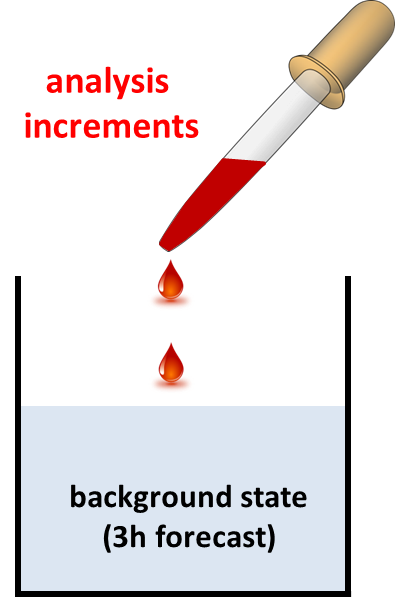
\includegraphics[width=0.30\textwidth]{analysis_drips.png}
 \caption{\textbf{I}ncremental \textbf{A}nalysis \textbf{U}pdate. Analysis increments are added to the background state (FG) in small drips over 
some time interval rather than in one go. Currently, increments for \texttt{U}, \texttt{V}, \texttt{P}, \texttt{T}, \texttt{QV} are treated in 
this way.}\label{fig_ana_drips}
\end{figure}

Mathematically speaking, during forward integration the model is forced with appropriately weighted analysis increments:
\begin{align}
 \frac{\mathrm{d} \mathbf{x}}{\mathrm{d} t} = A\mathbf{x} + g(t)\Delta\mathbf{x}^{A}\qquad \text{, with}\quad \int g(t)\, \mathrm{d}t = 1
\end{align}
$\mathbf{x}$ is the discrete model state, $A$ is a matrix representing the (non)-linear dynamics of the system and $g(t)$ is a weighting 
function, which is non-zero over some time-interval $\Delta t$.

This drip by drip incorporation acts as a low pass filter in frequency domain on the analysis increments such that 
small scale unbalanced modes are effectively filtered (see \cite{Bloom96}). The filter characteristic depends on the weighting function 
$g(t)$. It should be noted that IAU only filters the increments and not the backgound state, such that regions where analysis increments are 
zero remain unaffected. This method is currently applied to the prognostic atmospheric fields $\pi$, $\rho$, $v_{n}$, $q_{v}$, based on 
analysis increments provided for $u$, $v$, $p$, $t$ and $q_{v}$. $\pi$ denotes the Exner pressure.

The method sounds incredibly simple, however there are a few technical aspects to be taken care of when implementing this into an operational 
system: Figure \ref{fig_IAU_scheme} shows how the IAU-method is implemented in ICON for a $3\,\mathrm{h}$ assimilation run starting at midnight. 
Analysis increments are applied over a $3h$ hour time window, centered at the actual model start time. As indicated by the blue line, constant 
weights are used:
\begin{align}
 g(t) = \frac{\Delta t}{T}\qquad \text{, for } -T/2 < t < T/2
\end{align}
$T$ is the window width and $\Delta t$ is the fast physics time step. The key point in terms of technical implementation is that the model 
must be started $90$ minutes prior to the actual starting time of the assimilation run. The model is started from the 22:30 UTC first guess. 
The analysis increments for \texttt{U}, \texttt{V}, \texttt{P}, \texttt{T}, \texttt{QV}, whose validity time is 00:00 UTC are added over 
$3$ hours until at 1:30 the free forecast starts. Then, two first guess data sets are written into the database. One at 1:30 UTC, which will 
be used for starting the next 3h assimilation run, and a second one at 3:00 UTC, which serves as input for the assimilation system 
itself. Thus in general, using the IAU method requires some care in terms of reading and writing the right fields at the right times.
\begin{figure}[hbt]
 \centering
 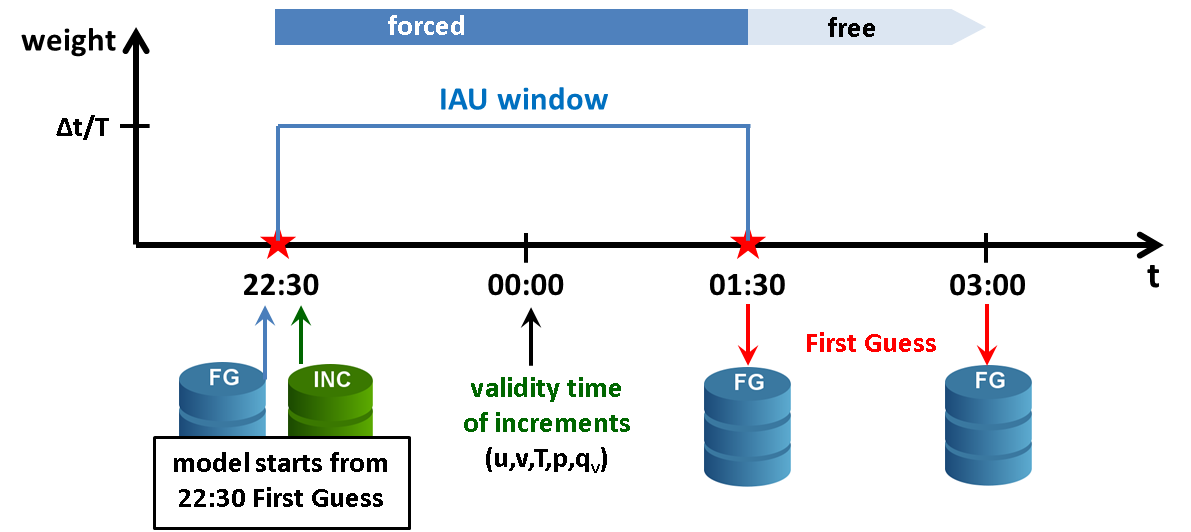
\includegraphics[width=1.0\textwidth]{IAU_scheme_2.png}
 \caption{Time line for an ICON assimilation run starting at 00:00 UTC.}\label{fig_IAU_scheme}
\end{figure}

%In principle, this method is not restricted to atmospheric fields, but also applicable to assimilated soil and surface fields. Possible candidates 
%would be: sea surface temperature \texttt{T\_SO(0)}, soil moisture \texttt{W\_SO}, 
